\documentclass{article}
\usepackage[margin=1in]{geometry}
\usepackage{setspace}
\usepackage{amsmath}
\usepackage{amssymb}
\usepackage{physics}
\usepackage{graphicx}
\usepackage{relsize}

\title{Math 180 Midterm 2}
\author{Jiaping Zeng}
\date{11/20/2020}

\begin{document}
\setstretch{1.5}

\newpage
\begin{itemize}
      \item [Q1]
            Prove the following statements using only the definition of a tree given in class and the lemmas regarding end-vertices. In particular, you may not use the Tree Characterization Theorem from class.
            \begin{enumerate}
                  \item Let $u$ and $v$ be distinct vertices of a connected graph $G$. Prove that if there exists more than one distinct path between $u$ and $v$, then $G$ contains a cycle.\\
                        \textbf{Answer}: Let $p_1$ and $p_2$ be two distinct paths between $u$ and $v$, we have the following two scenarios:
                        \begin{itemize}
                              \item [1.] $p_1$ and $p_2$ overlap on one or more vertices, but not all of them. Let $m,n\in \{u,v\}\cup p_1\cup p_2$ be two distinct vertices on both $p_1$ and $p_2$ such that there are two distinct paths $q_1$ and $q_2$ between $m$ and $n$ that does not overlap anywhere. Since $p_1$ and $p_2$ do not overlap on all vertices, such $m,n$ and $q_1,q_2$ always exists. Then $m\rightarrow q_1\rightarrow n\rightarrow q_2\rightarrow m$ forms a cycle.
                              \item [2.] $p_1$ and $p_2$ do not overlap anywhere, then $u\rightarrow p_1\rightarrow v\rightarrow p_2\rightarrow u$ is a cycle by definition.
                        \end{itemize}
                        Therefore $G$ must contain a cycle.
                  \item Let $G=(V,E)$ be a connected graph. Suppose $\abs{V}<\abs{E}+1$. Prove that $G$ contains a cycle.
                        \textbf{Answer}: Since $G$ is connected and has $\abs{V}$ vertices, it must have at least $\abs{V}-1$ edges, i.e. $\abs{E}\geq\abs{V}-1\implies\abs{V}\leq\abs{E}+1$. But by our assumption we cannot have $V=\abs{E}+1$, so we must add an edge to our minimally connected graph, which requires us to connected two distinct vertices $u,v$ that are not adjacent. Then this gives us two distinct paths between $u$ and $v$ and the previous part, $G$ must contain cycle.
            \end{enumerate}
\end{itemize}

\newpage
\begin{itemize}
      \item [Q2]
            Let $G(V,E)$ be the graph below. Let $X=V\cup E$ and consider the \textbf{incidence poset} $(X,\leq)$, where $x\leq y$ means ``$x=y$ or $x$ is the vertex incident to edge y.''
            \begin{center}
                  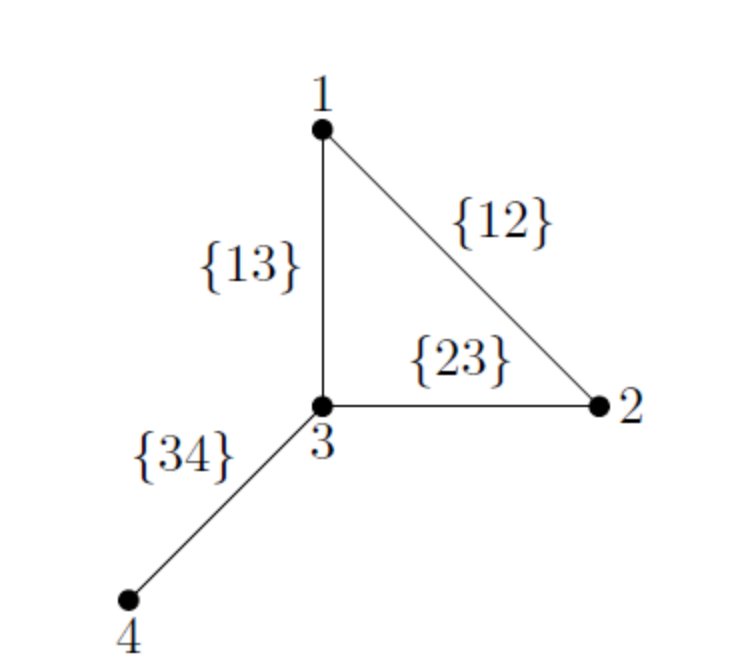
\includegraphics[width=2in]{q2.png}
            \end{center}
            \begin{enumerate}
                  \item Partition the elements of $X$ into the fewest number of disjoint chains possible.\\
                        \textbf{Answer}: We have $X=\{1,2,3,4,\{12\},\{13\},\{23\},\{34\}\}$, then we can partition it as $X=\{1,\{12\}\}\cup\{2,\{23\}\}\cup\{3,\{13\}\}\cup\{4,\{34\}\}$. This is the fewest number of disjoint chains possible as no two distinct vertices can be in the same chain; then since we have 4 vertices we have at least 4 disjoint chains.
                  \item Prove an upper bound for the longest antichain. Give an antichain of this length.\\
                        \textbf{Answer}: We can find the longest antichain by removing elements from $X$ such that none of the remaining vertices are connected to any edge. We can examine the following scenarios by the number of vertices removed:
                        \begin{enumerate}
                              \item we remove all vertices, in which case we can keep all the edges and have an antichain of length 4.
                              \item we remove 3 vertices, then we can keep the edges between the three, which gives us a maximal of 3 edges by removing vertices 1,2,3. So we have 1 vertex and 3 edges which gives us an antichain of length 4.
                              \item we remove 2 vertices, then we can only keep the one edge between them. Then we have an antichain of length 3.
                              \item we remove 1 vertex, then we still have to remove all edges, so we have an antichain of length 3.
                              \item we do not remove any vertex, then we must remove all the edges which gives us an antichain of length 4.
                        \end{enumerate}
                        Therefore the upperbound for the longest antichain is 4, with example $\{\{12\},\{13\},\{23\},\{34\}\}$ from the first scenario.
            \end{enumerate}
\end{itemize}

\newpage
\begin{itemize}
      \item [Q3]
            A \textbf{realizer} of a poset $(X,\leq)$ is a collection $F=\{L_1,L_2,\ldots,L_t\}$ of total orders of the elements of $X$ such that $(X,\leq)=\cap_{i=1}^t L_i$. In other words, $x<y$ in $(X,\leq)$ if and only if $x<y$ in every ordering $L_i$ in $F$. The \textbf{order dimension} of $(X,\leq)$ is the minimal $t$ such that $F=\{L_i,\ldots,L_t\}$ is realizer of $(X,\leq)$.\\
            A \textbf{total order} $(L_i,<_i)$ of $X$ is a chain containing every element of $X$.
            \begin{enumerate}
                  \item Prove that the order dimension of the incidence poset of a graph with more than one vertex is at least 2.\\
                        \textbf{Answer}: By contradiction. Suppose the incidence poset of a graph $G$ has an order dimension of 1. By definition, having an order dimension of 1 implies that $(X,\leq)=L_1$, where $L_1$ is a total order. However, since $G$ has more than one vertex, $L_1$ does not contain the two distinct vertices. Therefore $L_1$ is not a total order and the order dimension is at least 2.
                  \item Prove that the order dimension of the incidence poset of a path graph is at most 2. (The converse is true as well, but you do not need to prove this).\\
                        \textbf{Answer}: Since we have shown that the order dimension of a incidence poset on a graph is at least 2, we simply need to show that for a path graph, a collection $F=\{L_1,L_2\}$ of total orders always exists such that $(X,\leq)=L_1\cap L_2$. Take an arbitrary path $P_n$ with vertices $\{v_1,\ldots,v_n\}$, then we can construct one total order in one direction of the path, $L_1=v_1\leq v_2\leq v_1v_2\leq v_3\leq\ldots\leq v_n\leq v_{n-1}v_n$ (Note that the edges are shifted by 1 in the ordering, since we need to have both $v_i\leq v_iv_j$ and $v_j\leq v_iv_j$). Similarly, we can construct another total order in the opposite direction, $L_2=v_n\leq v_{n-1}\leq v_{n-1}v_n\leq v_{n-2}\leq\ldots\leq v_1\leq v_1v_2$. Then by construction we have $L_1\cap L_2=(X,\leq)$ and therefore the order dimension of  the incidence poset for a path graph is exactly 2.
                  \item \textbf{Claim:} The order dimension of the incidence poset of a graph $G$ (see Q2 above) is 3.\\
                        Prove the claim by giving three total orders $L_1,L_2,L_3$ which give a realizer of $(X,\leq)$.\\
                        \textbf{Answer}: By the converse of the previous part, since $G$ from Q2 is not a path graph, the order dimension of the incidence poset of it must be at least 3. We can show that the order dimension is exactly 3 by constructing $F=\{L_1,L_2,L_3\}$ as follows:\\
                        $L_1=1\leq 2\leq\{12\}\leq 3\leq 4\leq\{13\}\leq\{23\}\leq\{34\}$\\
                        $L_2=3\leq 1\leq\{13\}\leq 2\leq\{23\}\leq\{12\}\leq 4\leq\{34\}$\\
                        $L_3=4\leq 3\leq\{34\}\leq 2\leq\{23\}\leq 1\leq\{13\}\leq\{12\}$
            \end{enumerate}
\end{itemize}

\newpage
\begin{itemize}
      \item [Q4] Let $t\geq 2$ and $G=(V,E)$ be a graph on $n$ vertices with no subgraph isomorphic to $K_{2,t}$. Prove that \[\abs{E}\leq\frac{1}{2}(n^{\frac{t+1}{2}}+n)\]
            \textbf{Answer}: Let $V=V(G)$. For a fixed t-tuple, only one vertices $v\in V$ may exist joined to each of the vertices. If there were two such vertices, they would together with the t-tuple form a subgraph isomorphic to $K_{2,t}$. Hence $\abs{M}\leq\binom{n}{t}$.\\
            Now we can fix a vertex $v\in V$ and count the number of elements of the form $(\{u_1,\ldots,u_t\},v)$ that are contributed to the set $M$. For each t-tuple of its neighbors, $v$ contributes one elements of $M$, so if $v$ has degree $d$ it contributes $\binom{d}{2}$ elements. Therefore, if we denote by $d_1,d_2,\ldots,d_n$ the degrees of the vertices of $V$, we obtain $\abs{M}=\sum_{i=1}^n\binom{d_i}{2}$.\\
            So we have $\sum_{i=1}^n\binom{d_i}{2}\leq\binom{n}{t}$; by assuming that $G$ has no isolated vertices, i.e. $d_i\geq 1$ for all $i$, we have $\binom{d_i}{t}=\frac{d_i(d_i-1)}{2}\geq\frac{(d_i-1)^2}{2}$. Then, using the bound we found above, we have $\sum_{i=1}^n\frac{1}{2}(d_i-1)^2\leq\binom{n}{t}=\frac{n!}{t!(n-t)!}\leq\frac{n!}{2(n-t)!}$. Since $\frac{n!}{(n-t)!}\leq n^t$, we then have $\sum_{i=1}^n\frac{1}{2}(d_i-1)^2\leq\frac{n!}{2(n-t)!}\implies\sum_{i=1}^n(d_i-1)^2\leq n^t$.\\
            By applying Cauchy-Schwarz with $x_i=d_i-1$ and $y_i=1$, we have $\sum_{i=1}^n(d_i-1)\leq\sqrt{\sum_{i=1}^n(d_i-1)^2}\cdot\sqrt{\sum_{i=1}^n 1}\implies\sum_{i=1}^n(d_i-1)\leq\sqrt{n^t}\cdot\sqrt{n}\implies\sum_{i=1}^n d_i-\sum_{i=1}^n 1\leq\sqrt{n^t}\cdot\sqrt{n}\implies\sum_{i=1}^n d_i-n\leq\sqrt{n^{t+1}}\implies\sum_{i=1}^n d_i\leq n^{\frac{t+1}{2}}+n$. Then since $2\abs{E}=\sum_{i=1}^n d_i\implies\abs{E}=\frac{1}{2}\sum_{i=1}^n d_i$, we have $\abs{E}\leq\frac{1}{2}(n^{\frac{t+1}{2}}+n)$.
\end{itemize}

\newpage
\begin{itemize}
      \item [Q5]
            Construct the tree whose Prufer code is \[(5,2,6,5,9,2,2,9)\]
            \textbf{Answer}: We have $E=\{\{1,5\},\{3,2\},\{4,6\},\{6,5\},\{5,9\},\{7,2\},\{8,2\},\{2,9\},\{9,10\}\}$ by the Prufer code. Then the tree is as shown below:
            \begin{center}
                  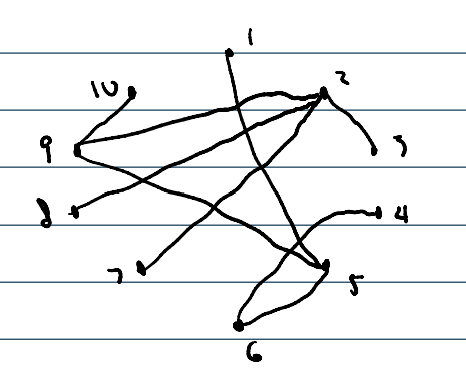
\includegraphics[width=3in]{5.png}
            \end{center}
\end{itemize}
\end{document}